\documentclass[11pt,a4paper]{article}
\usepackage[margin=1in]{geometry} % Adjust margins
\usepackage{authblk}
\usepackage{hyperref}
\usepackage{setspace}
\usepackage{amsmath, amssymb, amsthm}
\usepackage{graphicx}
\usepackage{float}
\usepackage{booktabs}
\usepackage{tabularx}
\usepackage{siunitx}
\usepackage{bm}

\setstretch{1.05} % Slightly tighter line spacing
\parskip=4pt      % Compact space between paragraphs
\renewcommand\Authfont{\normalsize}
\renewcommand\Affilfont{\itshape\small}

\title{\vspace{-1cm}Feature-Based Clustering of Time Series Using Ordinal Pattern Analysis\vspace{-0.3cm}}

\author[1]{M.\ H.\ M.\ R.\ S.\ Dilhani \thanks{Contact: \href{mailto:rasika.dilhani@vuw.ac.nz}{rasika.dilhani@vuw.ac.nz}}}
\author[1]{Alejandro C.\ Frery}
\author[2]{Andrea A.\ Rey}

\affil[1]{School of Mathematics and Statistics, Victoria University of Wellington, New Zealand}
\affil[2]{Laboratorio de Investigación y Desarrollo Experimental en Computación (LIDEC), Instituto de Tecnología e Ingeniería, Universidad Nacional de Hurlingham (UNAHUR), Argentina}

\date{}

\begin{document}
	\maketitle
	\vspace{-0.5cm}
	
	\begin{abstract}
	
	
Ordinal pattern analysis has emerged as a promising alternative to analysing time series data, providing a robust and computationally efficient approach. 
It involves converting time series data into a sequence of symbols that represent ordering relationships among data points within specific time windows.  
Then, the Shannon entropy and the Statistical Complexity are computed from the histogram of symbols. 
The method detects small differences between models and sample sizes.
We used ordinal pattern analysis to analyse simulated time series under Autoregressive (AR), Moving Average (MA), and Autoregressive Moving Average (ARMA) models. 
	
This study presents a simulation-based experiment into time series using ordinal pattern analysis. 
The primary research focus was on identifying the distinguishing characteristics of AR, MA, and ARMA models through ordinal patterns features. 
Simulated time series were generated with two series lengths ($n = 500$ and $n = 1000$), using parameter values chosen to satisfy the stationarity and invertibility conditions of the models. 
%%% ACF The table number does not show in my compiled PDF
The experimental design included several variants for each AR, MA, and ARMA model type, with each model representing a distinct parameter setting (Table~\ref{table:summary}). 
To ensure model accuracy, 100 independent replications were performed for each model configuration.

Ordinal patterns were extracted to compute entropy and complexity. 
Features were analysed in the entropy–complexity plane for model discrimination. 
ARMA(1,1) shows two distinct clusters.
AR coefficients $-0.8$ and $0.8$ produce lower entropy and higher complexity. 
Coefficients $0.1$ and $-0.1$ yield higher entropy and lower complexity. 
ARMA(2,2) shows overlapping groups across all four models. 
Clear separation appears by sample size, with larger samples forming more stable clusters. (Figures~\ref{fig:HC new n500} and \ref{fig:HC new n1000}).

%%% ACF Did you do anything related to clustering? 
The findings highlight the effectiveness of feature-based ordinal pattern analysis of time series, which uses Shannon entropy and complexity to characterize intrinsic differences among models. 
The simulation framework further validates the method’s reliability under varying structural and stochastic configurations. 
This research establishes a foundation for applying ordinal pattern analysis to unsupervised time series grouping, with potential applications in data-rich domains such as finance, engineering, and bioinformatics.

\end{abstract}

\begin{table}[hbt]
	\centering
	\begin{tabular}{llllll}
		\toprule
		\textbf{Type} & \textbf{Model} & $\alpha_1$ & $\alpha_2$ & $\beta_1$ & $\beta_2$ \\
		\midrule
		AR(1)      & AR1\_M1  & $0.8$   &      &      &      \\
		& AR1\_M2  & $0.1$   &      &      &      \\
		& AR1\_M3  & $-0.8$  &      &      &      \\
		& AR1\_M4  & $-0.1$  &      &      &      \\
		AR(2)      & AR2\_M1  & $0.1$   & $0.8$  &      &      \\
		& AR2\_M2  & $-0.8$  & $0.1$  &      &      \\
		& AR2\_M3  & $0.1$   & $-0.8$ &      &      \\
		& AR2\_M4  & $-0.8$  & $-0.1$ &      &      \\
		MA(1)      & MA1\_M1  &       &      & $0.8$  &      \\
		& MA1\_M2  &       &      & $0.1$  &      \\
		& MA1\_M3  &       &      & $-0.8$ &      \\
		& MA1\_M4  &       &      & $-0.1$ &      \\
		MA(2)      & MA2\_M1  &       &      & $0.1$  & $0.8$  \\
		& MA2\_M2  &       &      & $-0.8$ & $0.1$  \\
		& MA2\_M3  &       &      & $0.1$  & $-0.8$ \\
		& MA2\_M4  &       &      & $-0.8$ & $-0.1$ \\
		ARMA(1,1)  & ARMA11\_M1 & $0.8$ &      & $0.8$  &      \\
		& ARMA11\_M2 & $0.1$ &      & $0.1$  &      \\
		& ARMA11\_M3 & $-0.8$ &     & $-0.8$ &      \\
		& ARMA11\_M4 & $-0.1$ &     & $-0.1$ &      \\
		ARMA(2,2)  & ARMA22\_M1 & $0.1$ & $0.8$  & $0.1$  & $0.8$  \\
		& ARMA22\_M2 & $-0.8$ & $0.1$ & $-0.8$ & $0.1$  \\
		& ARMA22\_M3 & $0.1$ & $-0.8$ & $0.1$  & $-0.8$ \\
		& ARMA22\_M4 & $-0.8$ & $-0.1$ & $-0.8$ & $-0.1$ \\
		\bottomrule
	\end{tabular}
	\caption{Models and parameter sets for AR(1), AR(2), MA(1), MA(2), ARMA(1,1), and ARMA(2,2). Empty cells indicate omitted parameters.}
	\label{table:summary}
\end{table}

\begin{figure}[H]
	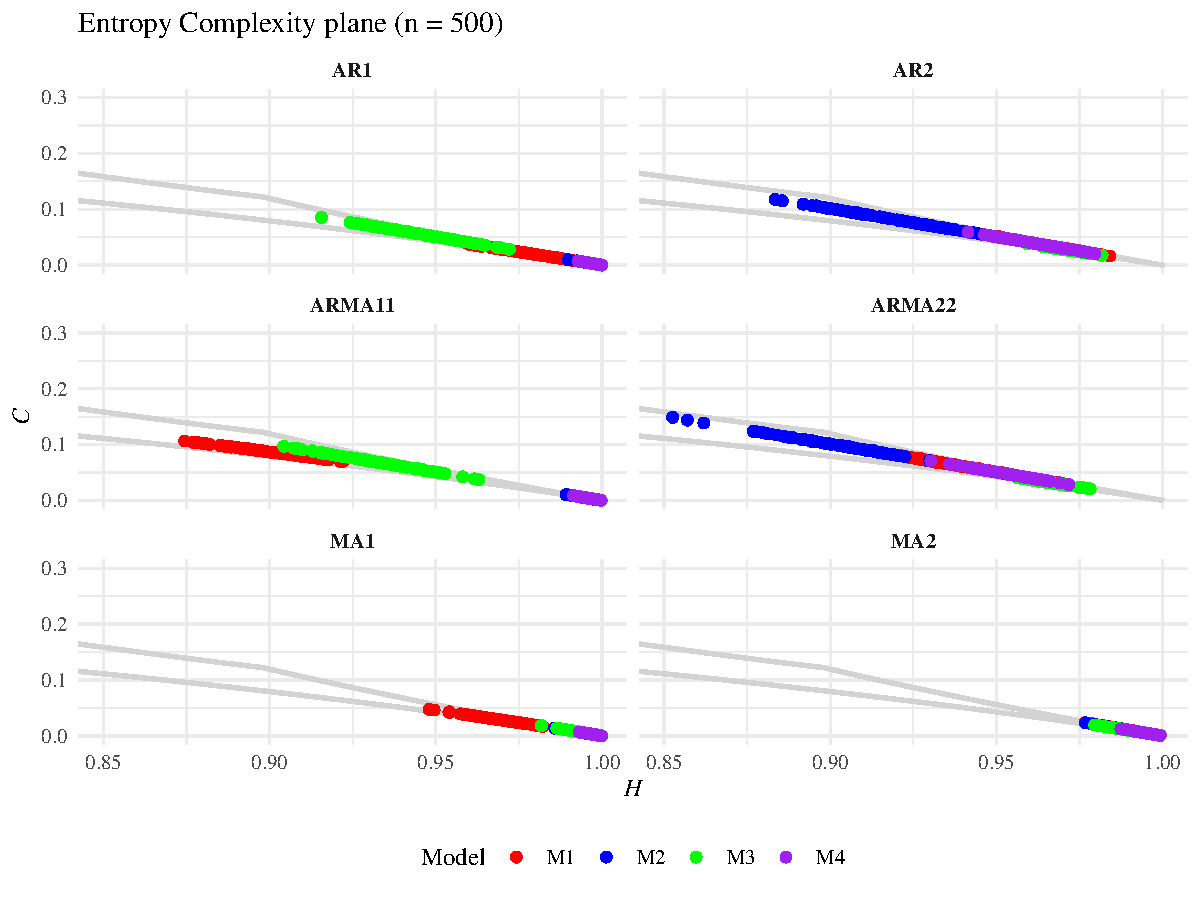
\includegraphics[width=0.9 \textwidth]{New_model_group_plot_n500}
	\caption{$H \times C$ plane for new model n500}
	\label{fig:HC new n500}
\end{figure}

\begin{figure}[H]
	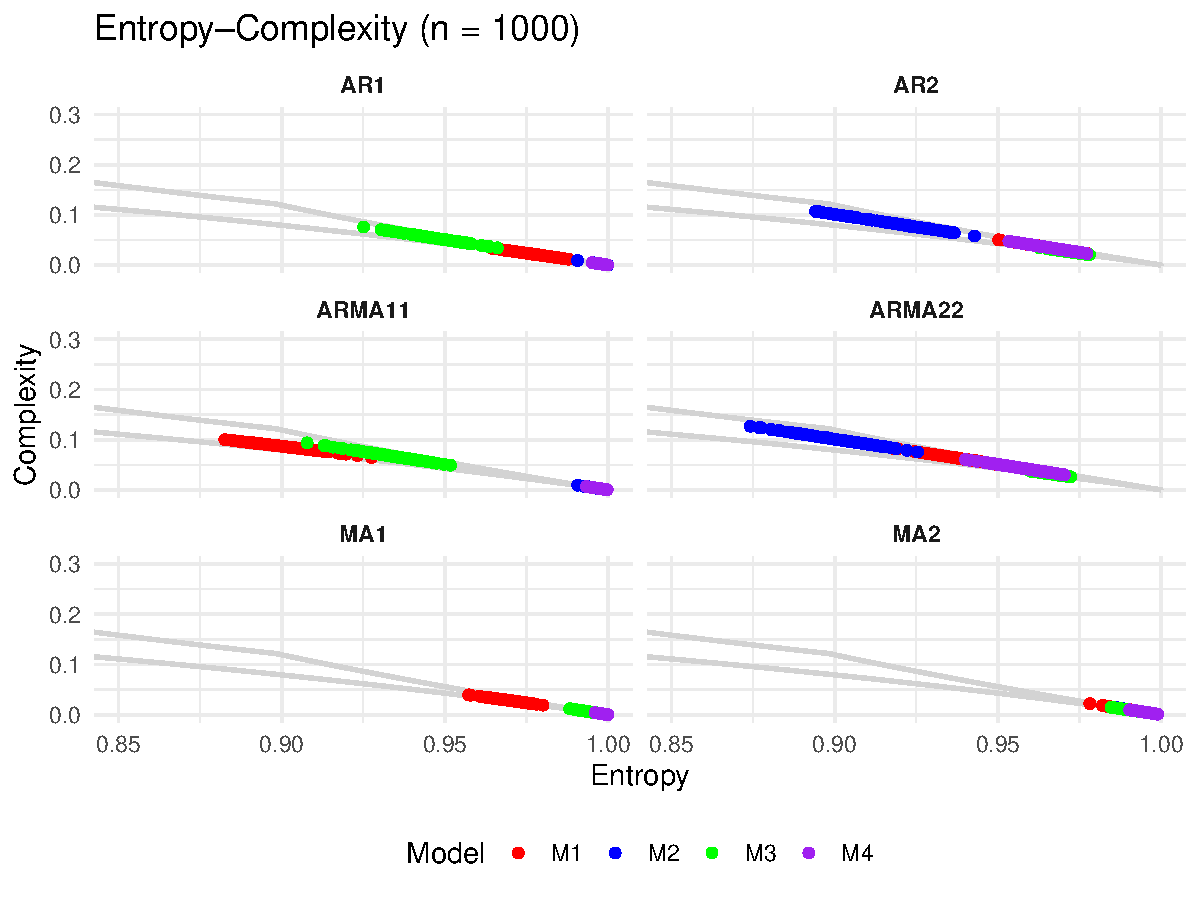
\includegraphics[width=0.9 \textwidth]{New_model_group_plot_n1000}
	\caption{$H \times C$ plane for new model n1000}
	\label{fig:HC new n1000}
\end{figure}


\end{document}

